
    \documentclass{article}
    \usepackage[T2A]{fontenc}
    \usepackage[utf8]{inputenc}
    \usepackage[russian]{babel}
    \title{test}
    \usepackage{graphicx}
    \graphicspath{ {artifacts/} }
    \author{Слава Плеханов}
    
    \begin{document}
    \begin{center}
        Amazing Table:
    \end{center}
\begin{tabular}{ | l | l | l | }
\hline
Writer & Year of birth & Country of birth \\ \hline
Dovlatov & 1941 & USSR\\
Pelevin & 1962 & USSR\\
Lem & 1962 & Poland\\
Sholohov & 1905 & Russian Empire\\
Remark & 1898 & Germany\\
Strugatsky & 1925 \& 1933 & USSR\\
\hline\end{tabular}
    \hfill \break
    \hfill \break
    \hfill \break
    \hfill \break
    \hfill \break

    \begin{center}
        Fantastic Picture:
    \end{center}
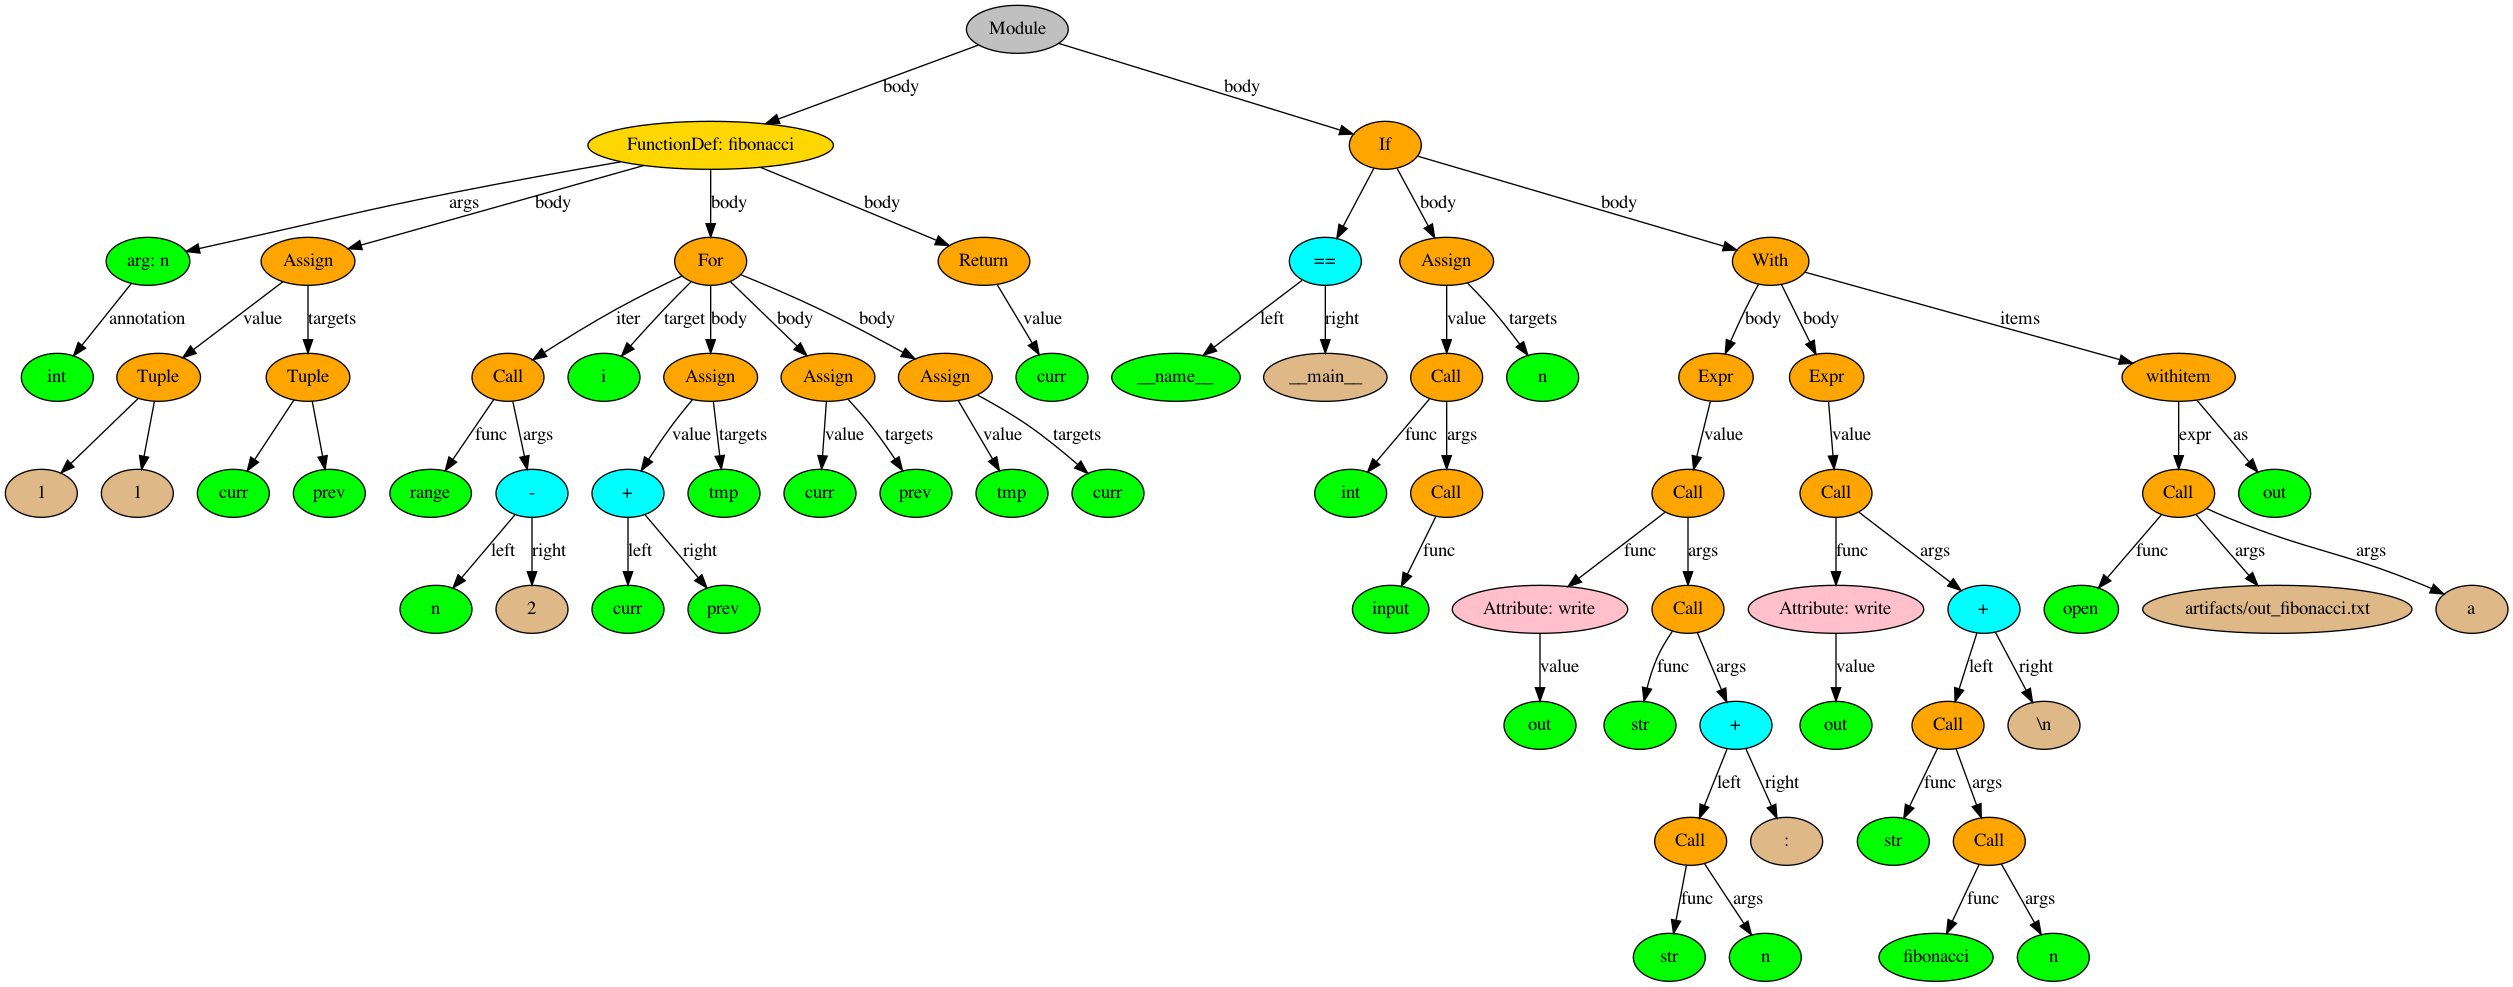
\includegraphics[scale=0.15]{tree.png}\end{document}
\hline
\end{tabular}
\end{document}
